\documentclass[11pt]{scrartcl}
\usepackage{dominatrix}
\usepackage{solarized-light}
\lstset{
language=R
}

\newcommand{\sgn}{\ensuremath{\mathrm{sgn}}}

\usepackage{dsfont}

\title{Homework 2}
\subject{Statistical Machine Learning (STAT W4400)}
\author{Linan Qiu\\\texttt{lq2137}}
\begin{document}
\maketitle

\textbf{Note: since submission only allows \texttt{.pdf} and \texttt{.R}, I did not preserve the directory structure of this project. The \texttt{.R} files will not run properly due to imports and assumed directory structure. For a functional version, go to \url{https://github.com/linanqiu/stat-w4400-homework/tree/master/hw2/r}}

\section{Linear Classification}

\subsection{Classification Results}

$\mathbf{v}_h$ is a unit vector.

\begin{lstlisting}
vh = matrix(c(1/sqrt(2), 1/sqrt(2)), nrow=2)
c = 1/(2 * sqrt(2))
x1 = matrix(c(-3, 0), nrow=2)
x2 = matrix(c(1/2, 1/2), nrow=2)

> sign(crossprod(x1, vh) - c)
     [,1]
[1,]   -1
> sign(crossprod(x2, vh) - c)
     [,1]
[1,]    1
\end{lstlisting}

\[r_1 = \sgn(<\mathbf{x}_1, \mathbf{v}_h> - c) = -1 \]
\[r_1 = \sgn(<\mathbf{x}_2, \mathbf{v}_h> - c) = 1 \]

\subsection{SVM with Margin}

Concept of margin applies only to training, not classification. Classification works for any linear classifier. For the test point $\mathbf{x}$,

\[r = \sgn(<\mathbf{x}_1, \mathbf{v}_h> - c)\]

still applies. Hence the predicted classes will still be the same.

\subsection{Cost Function Approximated by Perceptron Cost Function}

It approximates the empirical risk function. Empirical risk function is piece-wise constant, hence would not allow us to gradient descent optimally. The perceptron cost function, by using $\left|\left<\mathbf{z} ,\begin{pmatrix}1 \\ \tilde{\mathbf{x}}_i \end{pmatrix}\right>\right|$ instead of just the loss function.

\section{Perceptron}

\subsection{Classify}

Included in file \texttt{problem2.R}

\subsection{Perceptron Training Algorithm}

Included in file \texttt{problem2.R}

\subsection{Train and Test}

Included in file \texttt{problem2.R}

\subsection{2D Representation}

Slope can be obtained from $\mathbf{v}_h$ by

\[v_x x + v_y y - c = 0\]

and solving accordingly.

\begin{figure}[H]
\centering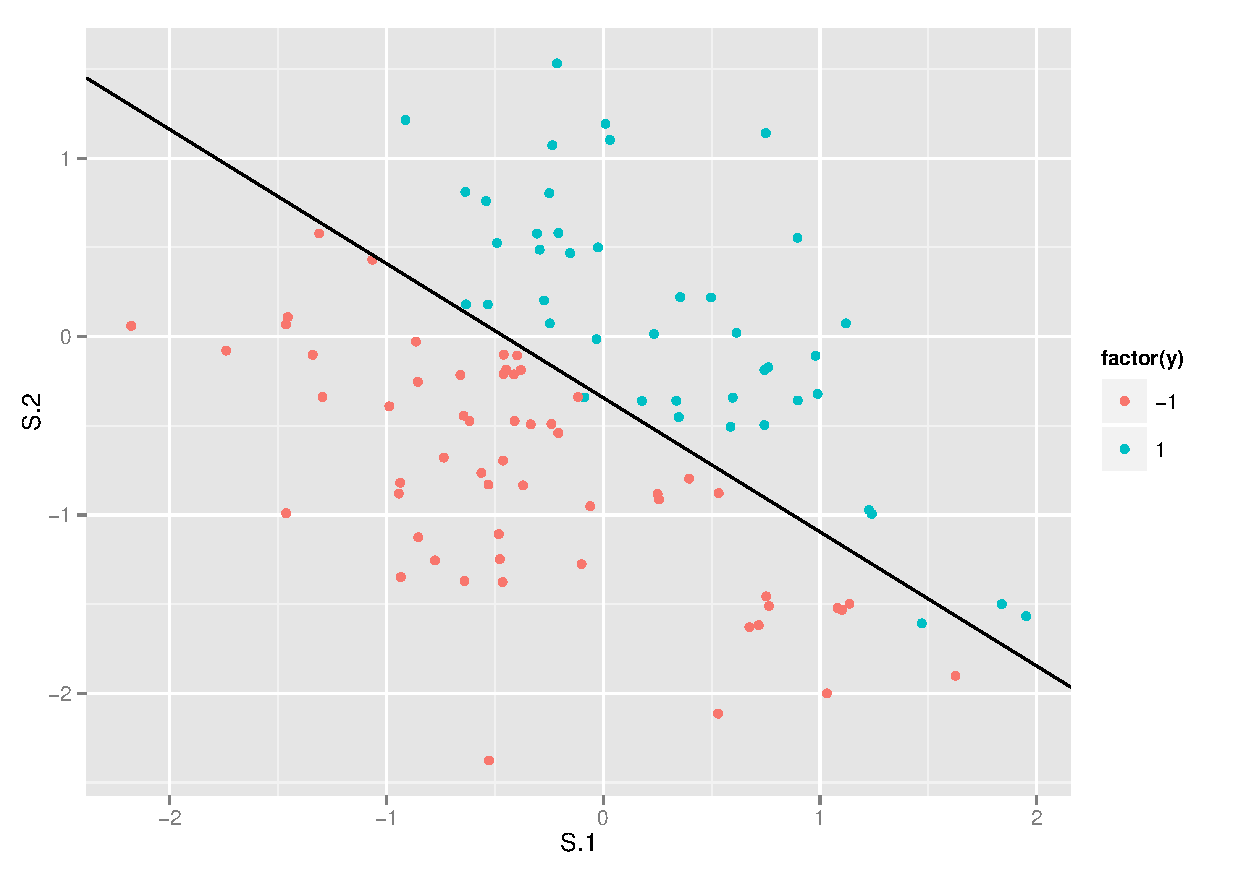
\includegraphics[width=\textwidth]{./hw2/r/test.pdf}
\caption{Plot of test data against obtained classifier from \texttt{z}.}
\end{figure}

\begin{figure}[H]
\centering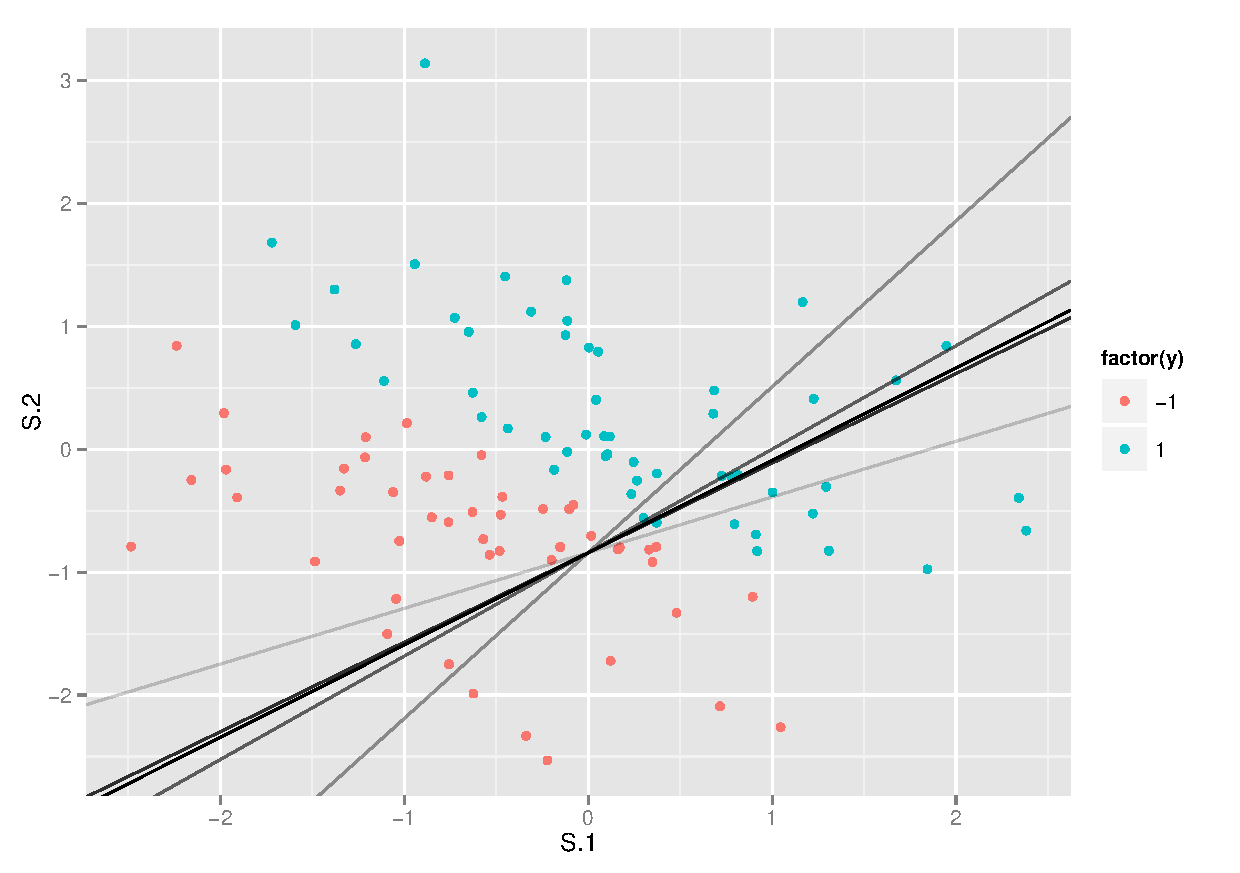
\includegraphics[width=\textwidth]{./hw2/r/train.pdf}
\caption{Plot of training data against history of classifiers from \texttt{z\_history}. Earlier iterations have lower alpha.}
\end{figure}

\section{SVM}

\subsection{Cross Validation Estimates}

\begin{figure}[H]
\centering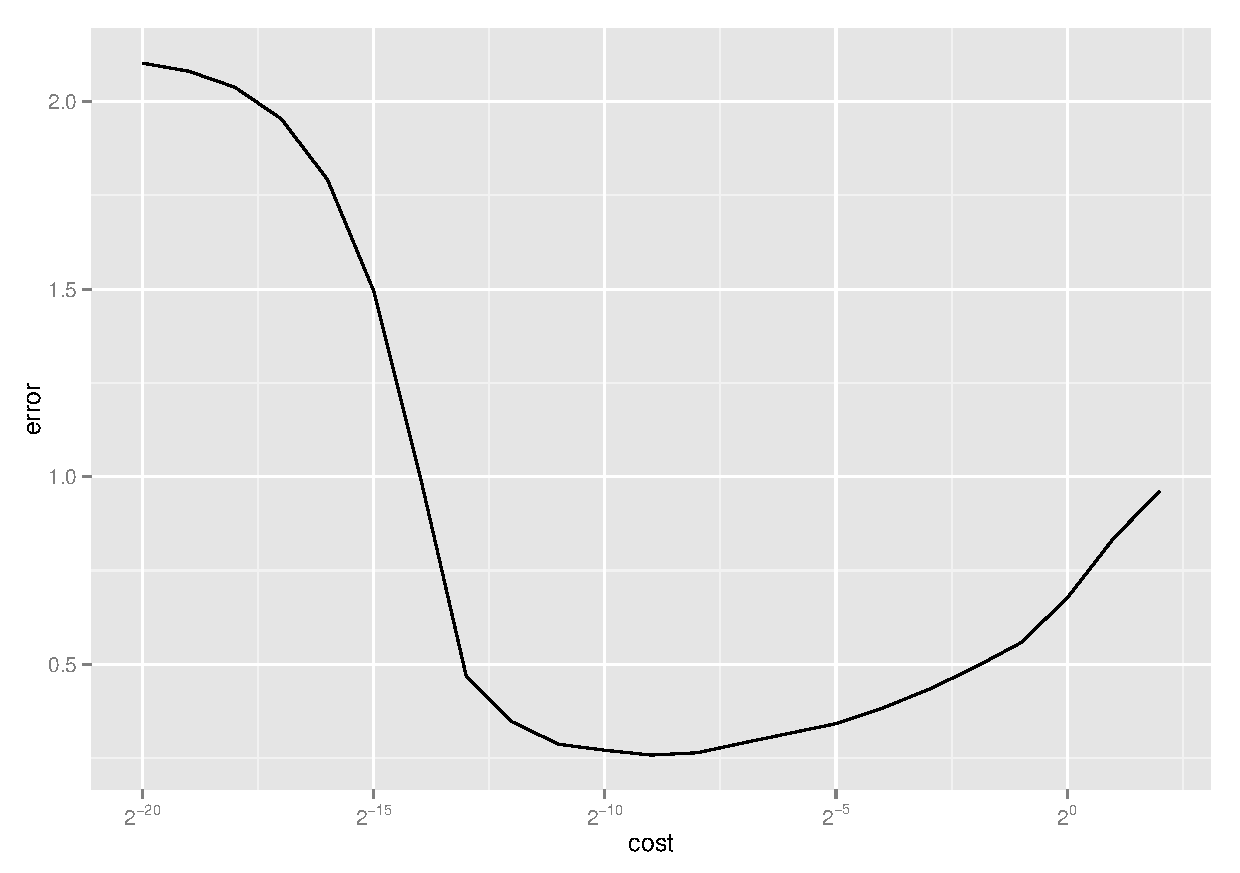
\includegraphics[width=\textwidth]{./hw2/r/tune_linear.pdf}
\caption{Plot of error against margin parameter (cost) for linear kernel SVM}
\end{figure}

\begin{figure}[H]
\centering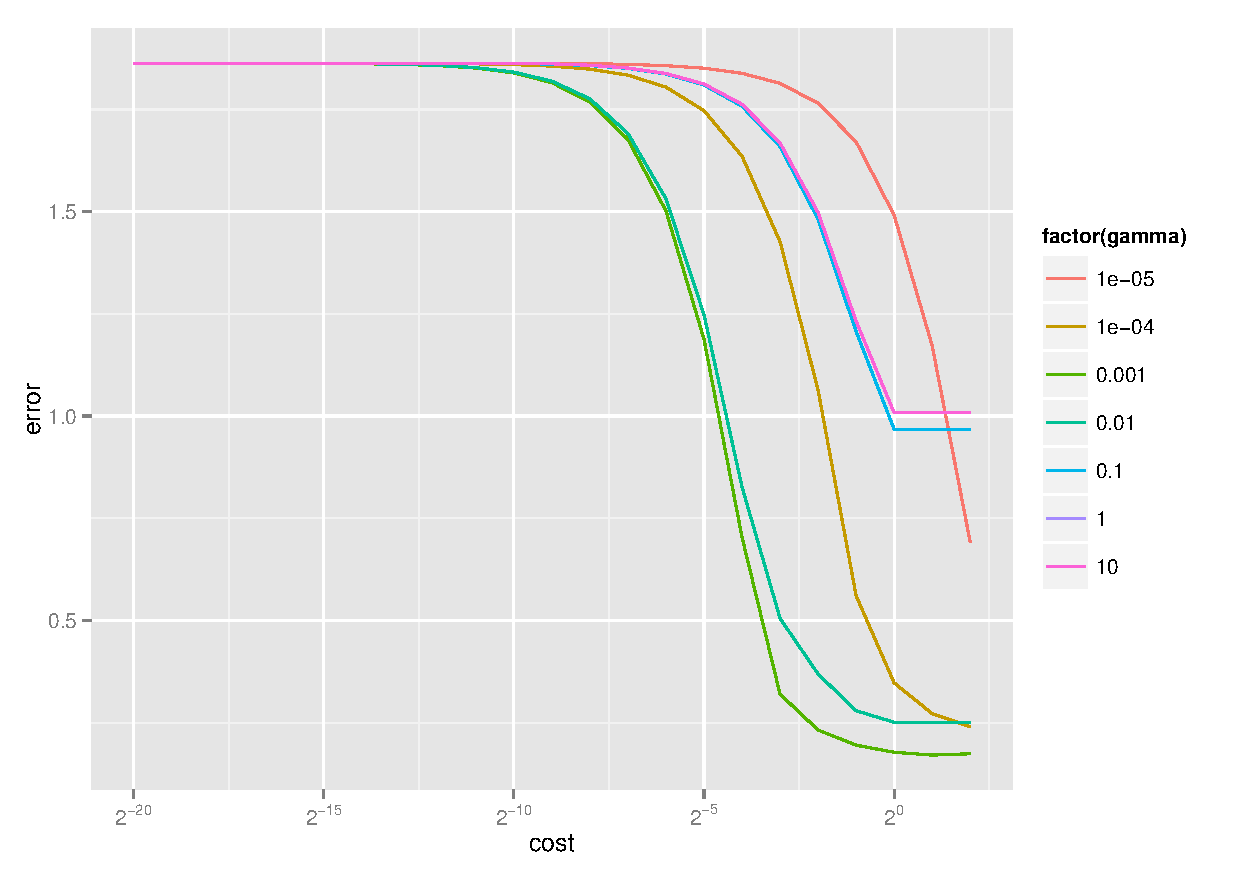
\includegraphics[width=\textwidth]{./hw2/r/tune_rbf.pdf}
\caption{Plot of error against margin parameter (cost) for different kernel bandwidth (gamma) for RBF kernel SVM}
\end{figure}

\subsection{Test}

Selected parameter values are:

\begin{lstlisting}
> tuned_linear

Parameter tuning of 'svm':

- sampling method: 10-fold cross validation 

- best parameters:
        cost
 0.001953125

- best performance: 0.025 

> tuned_rbf

Parameter tuning of 'svm':

- sampling method: 10-fold cross validation 

- best parameters:
 gamma cost
 0.001  0.5

- best performance: 0.01875 
\end{lstlisting}

It seems from the training data tuning that the RBF kernel has a better performance. However, upon testing, this is not immediately clear.

\begin{lstlisting}
> linear_model = svm(labels ~ ., data=data, method="C-classification", kernel="linear", cost=tuned_linear$best.parameter$cost[1])
> linear_predict = predict(linear_model, testset[, -ncol(data)])
> classAgreement(table(pred = linear_predict, true = testset[, ncol(data)]))
$diag
[1] 0.975

$kappa
[1] 0.9497487

$rand
[1] 0.95

$crand
[1] 0.8999645

> 
> rbf_model = svm(labels ~ ., data=data, method="C-classification", kernel="radial", cost=tuned_rbf$best.parameter$cost[1], gamma=tuned_rbf$best.parameter$gamma[1])
> rbf_predict = predict(rbf_model, testset[, -ncol(data)])
> classAgreement(table(pred = rbf_predict, true = testset[, ncol(data)]))
$diag
[1] 0.975

$kappa
[1] 0.9497487

$rand
[1] 0.95

$crand
[1] 0.8999645
\end{lstlisting}

Both models give the same accuracy rate (hence misclassification rate).

\end{document}
